\setchapterpreamble[u]{\margintoc}
\chapter{Sensitivity of IceCube-Gen2 to measure flavour composition of Astrophysical Neutrinos}
\labch{gen2}
This chapter details the sensitivity studies performed for \emph{The IceCube Gen2 detector}. A siginificant portion of this thesis work was dedicated to assess and derive sensitivity to measure the flavour composition of Astrophysical Neutrinos for IceCube Gen2. The detector will be introduced in the following sections, along with the simulations and software framework used to produce the results. 

\section{IceCube Gen2} 
\label{sec:gen2-detector}
IceCube-Gen2 is a proposed next generation of neutrino detector, designed to observe the neutrino sky within a wide energy range, from TeV to EeV \sidecite{whitepaper}. Its sensitivity is expected to be at least five times better than IceCube, enabling the observation of individual sources. The instrument layout is designed to detect about ten times more neutrinos annually as compared to IceCube. This increased capability will facilitate in-depth studies of neutrino distribution across the sky, energy spectrum, and flavor composition and beyond standard model physics.
\begin{figure}[h!]
	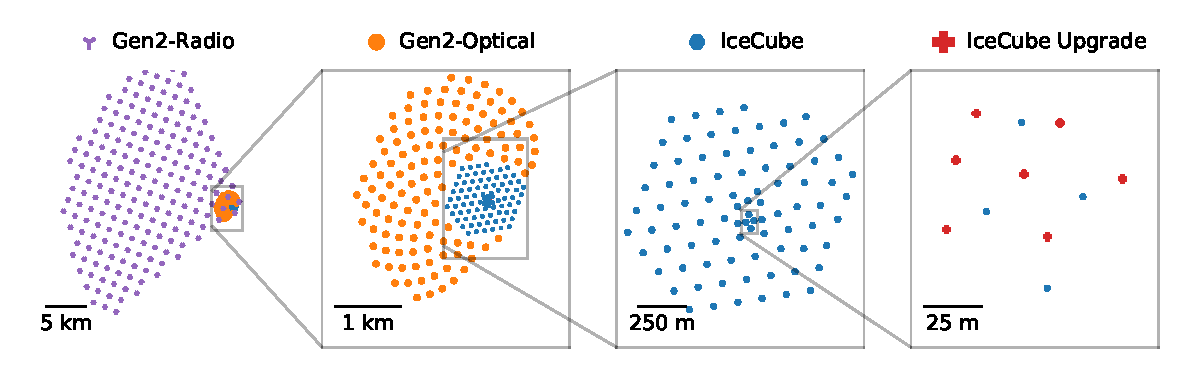
\includegraphics[scale=1.5]{./figures/gen2/decadal_survey_gen2-fan_radio_geometry.pdf}
	\caption{Figure depicts the proposed IceCube-Gen2 Neutrino Observatory facility at the South Pole. It includes (from left to right) (i) a radio array with 200 stations, (ii) 120 new in-ice strings, spaced 240 m apart (shown as orange points), as an expansion of (iii) current optical array, (iv) 7 strings of IceCube upgrade, to be deployed soon within currrent in-ice DeepCore volume. Figure taken from \cite{whitepaper}}
	\labfig{gen2_all_geometry}
\end{figure}

\reffig{gen2_all_geometry} illustrates a top view of the IceCube-Gen2 facility, showcasing its various components using optimized technologies for the targeted energy ranges. 

\begin{description}
    \item \textbf{\emph{The IceCube Upgrade}} will start deployment this season. Its goal is to lower the detection threshold for neutrinos to 1 GeV (In-line with its predecessor, \emph{DeepCore} in current IceCube)\todo{cite Upgrade paper, ICRC 2019 from Aya?}. This improvement will advance oscillation measurements, dark matter searches, and studies of physics beyond the Standard Model. The IceCube Upgrade project will also deploy 693 new types of multi-PMT detector modules, providing an opportunity to test the optical sensor technology for the IceCube-Gen2 observatory.

    \item \textbf{\emph{The surface array}} of IceCube-Gen2 is a unique setup where the surface array measures the electromagnetic shower component and low-energy muons, while the optical array detects TeV and potentially PeV muons from the same air shower \sidecite{IceCubeCollaborationSchroeder2024_1000168735}. Planned to be used similarly as \emph{IceTop} of IceCube, the stations shall be placed on top of the additional \emph{in-ice} strings of optical array. It can also be used as \emph{surface veto} to reduce the background of atmospheric muons in samples of astrophysical neutrinos from the southern sky.

    \item \textbf{\emph{The Radio array}} aims to discover and characterize high-energy neutrino flux above 10 PeV. It detects nanosecond-scale radio emissions from ultra-high-energy particle showers using the Askaryan effect \sidecite{Askaryan,meyers_21}. This technique is sensitive to energies above PeV and complements the energy range of the optical array by capturing radio emissions from neutral and charged-current interactions, as well as energy losses of secondary leptons. 

    \item \textbf{\emph{The optical array}} includes addition of 120 new strings to the existing IceCube strings with an average horizontal spacing of 240 m arranged in what is reffered to as \emph{sunflower geometry}. Both, the shape and of the array and spacing between the strings were derived by doing dedicated geometry optimization studies \sidecite{Geometry_optimization,Anastasiia}. Each string hosts 80 modules, totaling 9600 new modules, placed between 1325 m and 2575 m below the surface. Vertical spacing between modules amounts to 16 m, resulting in an instrumented geometric volume of 7.9 $\mathrm{km}^3$. Each module on the string is assumed to collect nearly three times as many photons as an IceCube DOM. \todo{cite TDR link here? or is whitepaper ok?}
\end{description}

For the sensitivity study presented in this thesis, only the optical part of the proposed detector was simulated and used. 

\section{Simulation}
\label{sec:gen2-sim}
To perform this sensitivity study, dedicated simulations were carried out. The study aims not only to assess the sensitivity of IceCube-Gen2 in measuring the flavor composition of astrophysical neutrinos but also to evaluate its capabilities in detecting tau neutrino events, which is a crucial component as described in \ref{nu_samples}. The simulations were aligned with the mainline IceCube simulations (detailed in \ref{nu_samples} \todo{cite the simulation section here and not the chapter}) to enable direct comparisons. However, necessary modifications were made to account for the new-generation optical sensors to be used in IceCube Gen2 and the sparser geometry. The following sections will describe the event samples created using these simulations to conduct the sensitivity analysis.

\subsection{Isotropic Sensor}
\label{sec:isopdom}
The optical sensors to be used in the IceCube-Gen2 project depends a lot on how well the reference optical sensors to be deployed in the IceCube upgrade perform.\sidecite{Gen2_TDR}. The designs have been carefully optimized to balance cost-effectiveness, logistical efficiency, and enhanced performance. \reffig{Gen2DOMs} shows both the 16 and 18 PMT modules, which are being considered to use in IceCube Gen2, along with \textbf{mDOM} (\emph{multi PMT Digital Optical Module}) \sidecite{mDOM_2017,mDOM_2019} and \textbf{D-Egg} (\emph{Dual optical sensors in an Ellipsoid Glass for Gen2}) \sidecite{D-Egg_MainPaper} that are to be deployed in ice for IceCube Upgrade.

\begin{figure}
	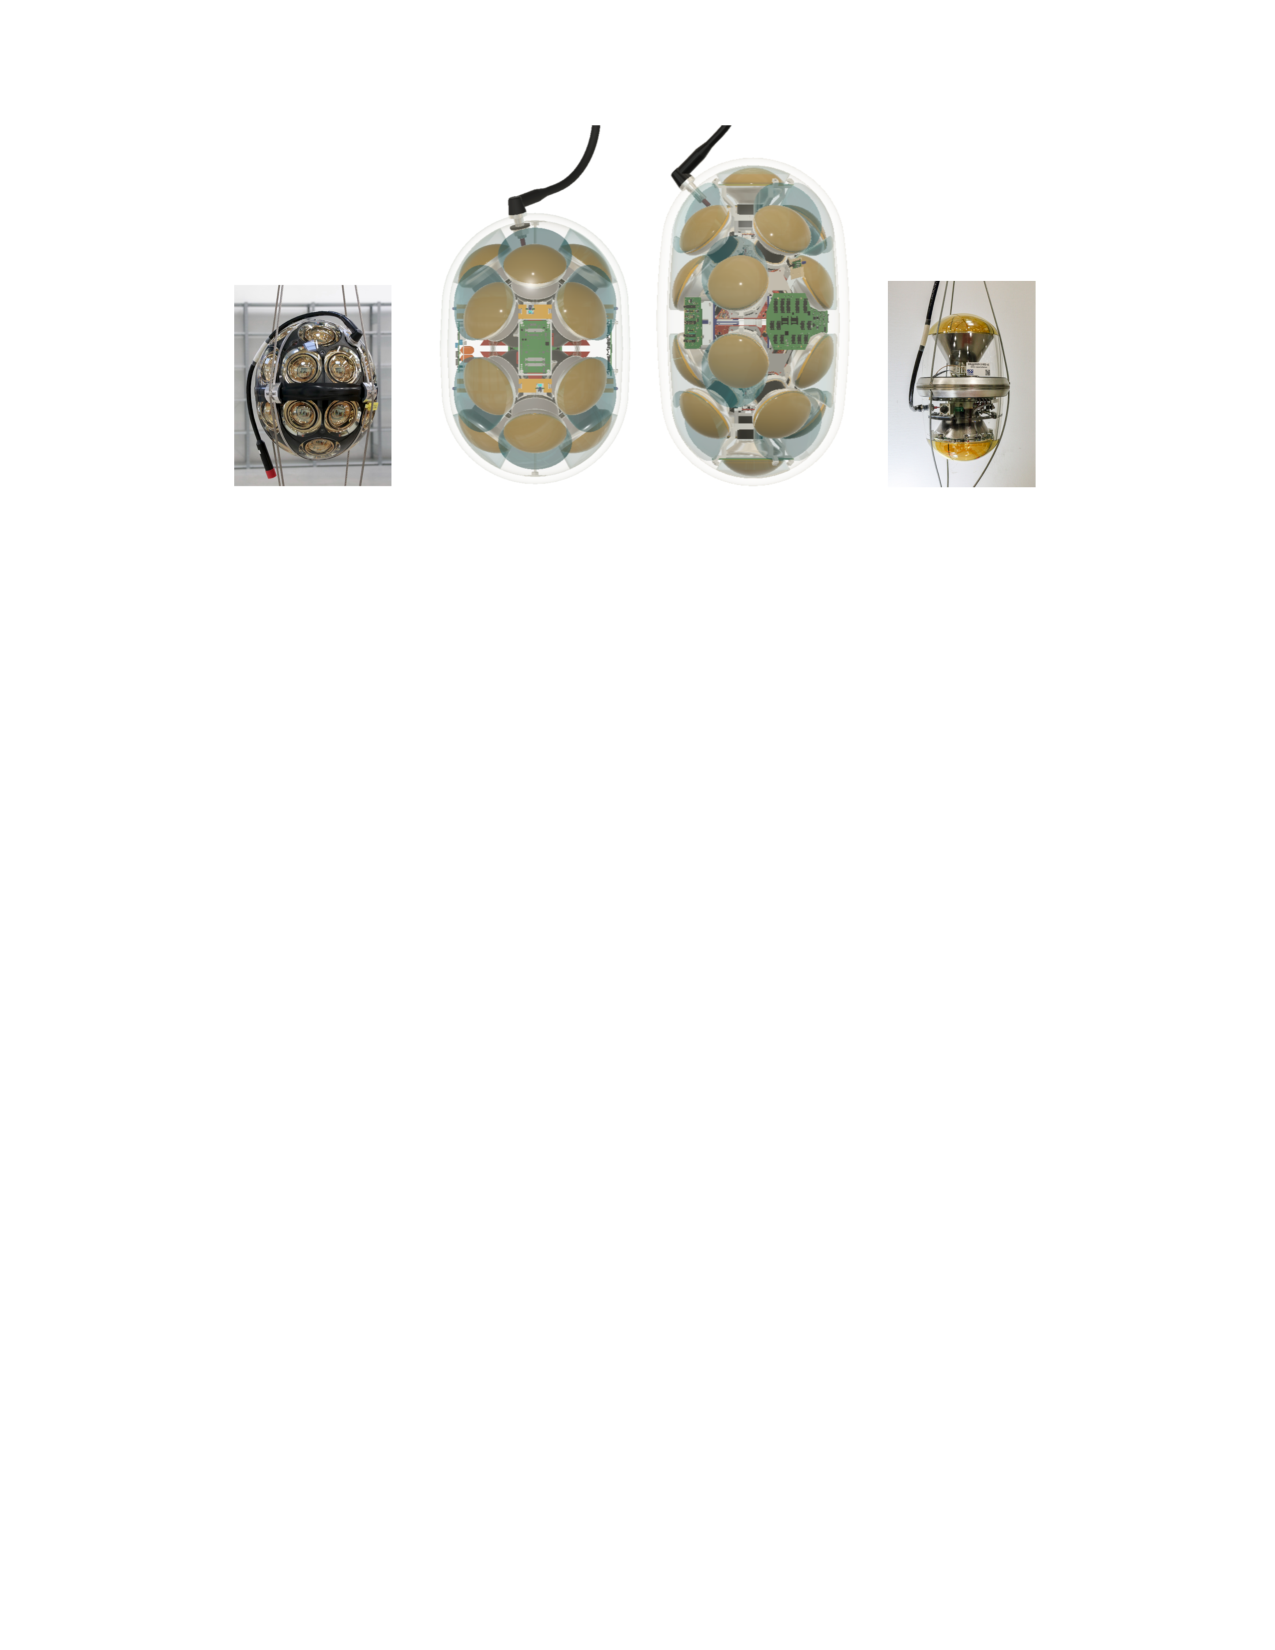
\includegraphics[scale=2.2]{./figures/gen2/Gen2_DOMs.pdf}
	\caption{The designs of the IceCube-Gen2 optical sensors, DOM-16(second) and DOM-18 (third) with their base designs, to be used in the IceCube Upgrade sensors, are the mDOM on the left and D-Egg on the right \cite{Gen2_TDR}}
	\labfig{Gen2DOMs}
\end{figure}



% \todo{did this project eventually become Upgrade?}

The simulations produced for this study includes the shape and characteristics of a module like the mDOM. Unlike IceCube’s single large 10" PMT, the mDOM consists of 24 smaller 3" PMTs. The key advantages of the mDOM over pDOM are its 2.2 times higher effective photocathode area, omnidirectional sensitivity, and the directional information obtained from the individual “pixels” (the 24 PMTs). Due to the large number of PMTs and their strategic placement within the module sphere, this module offers nearly isotropic angular acceptance, unlike IceCube DOMs with only one downward-facing PMT. 
\begin{marginfigure}
    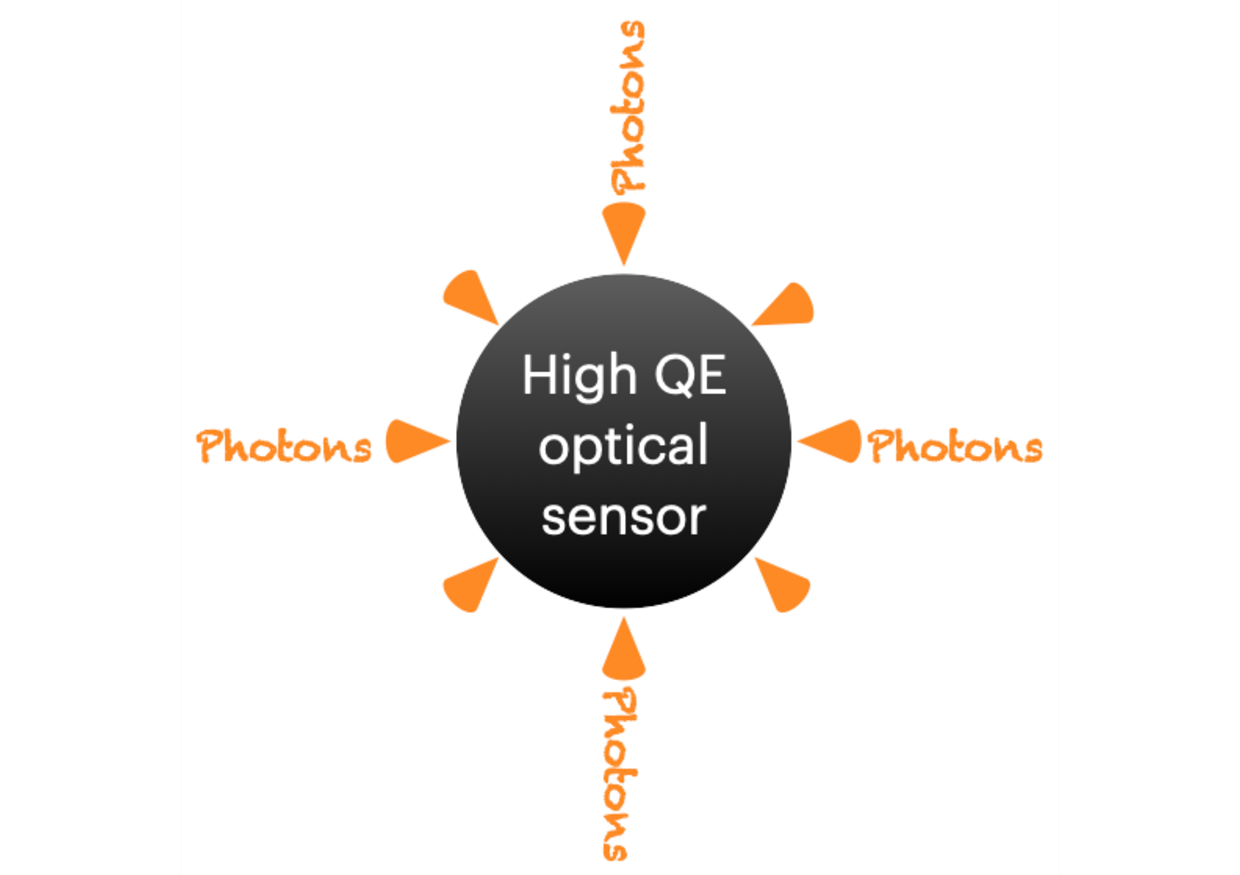
\includegraphics{./figures/gen2/iso-pDOM.pdf}
    \caption{Conceptual representation of Simulated sensor with isotropic angular acceptance (iso-pDOM)}
    \labfig{isoPDOM_schematic}
\end{marginfigure}
\marginnote{
    \begin{kaobox}[title=pDOM]
        pDOM stands for PINGU Digital Optical Module. It was first coined for an R\&D upgrade of IceCube DeepCore called \textbf{PINGU} (The Precision IceCube Next Generation Upgrad) \cite{PINGU}. pDOM has a High Quantum Efficiency PMT, making it very similar to DOMs in IceCube DeepCore. The key design difference was to have a single "Main board" instead of various boards on the DOM, making the overall processing much simpler and faster. 
    \end{kaobox}}
% \begin{marginfigure}
%     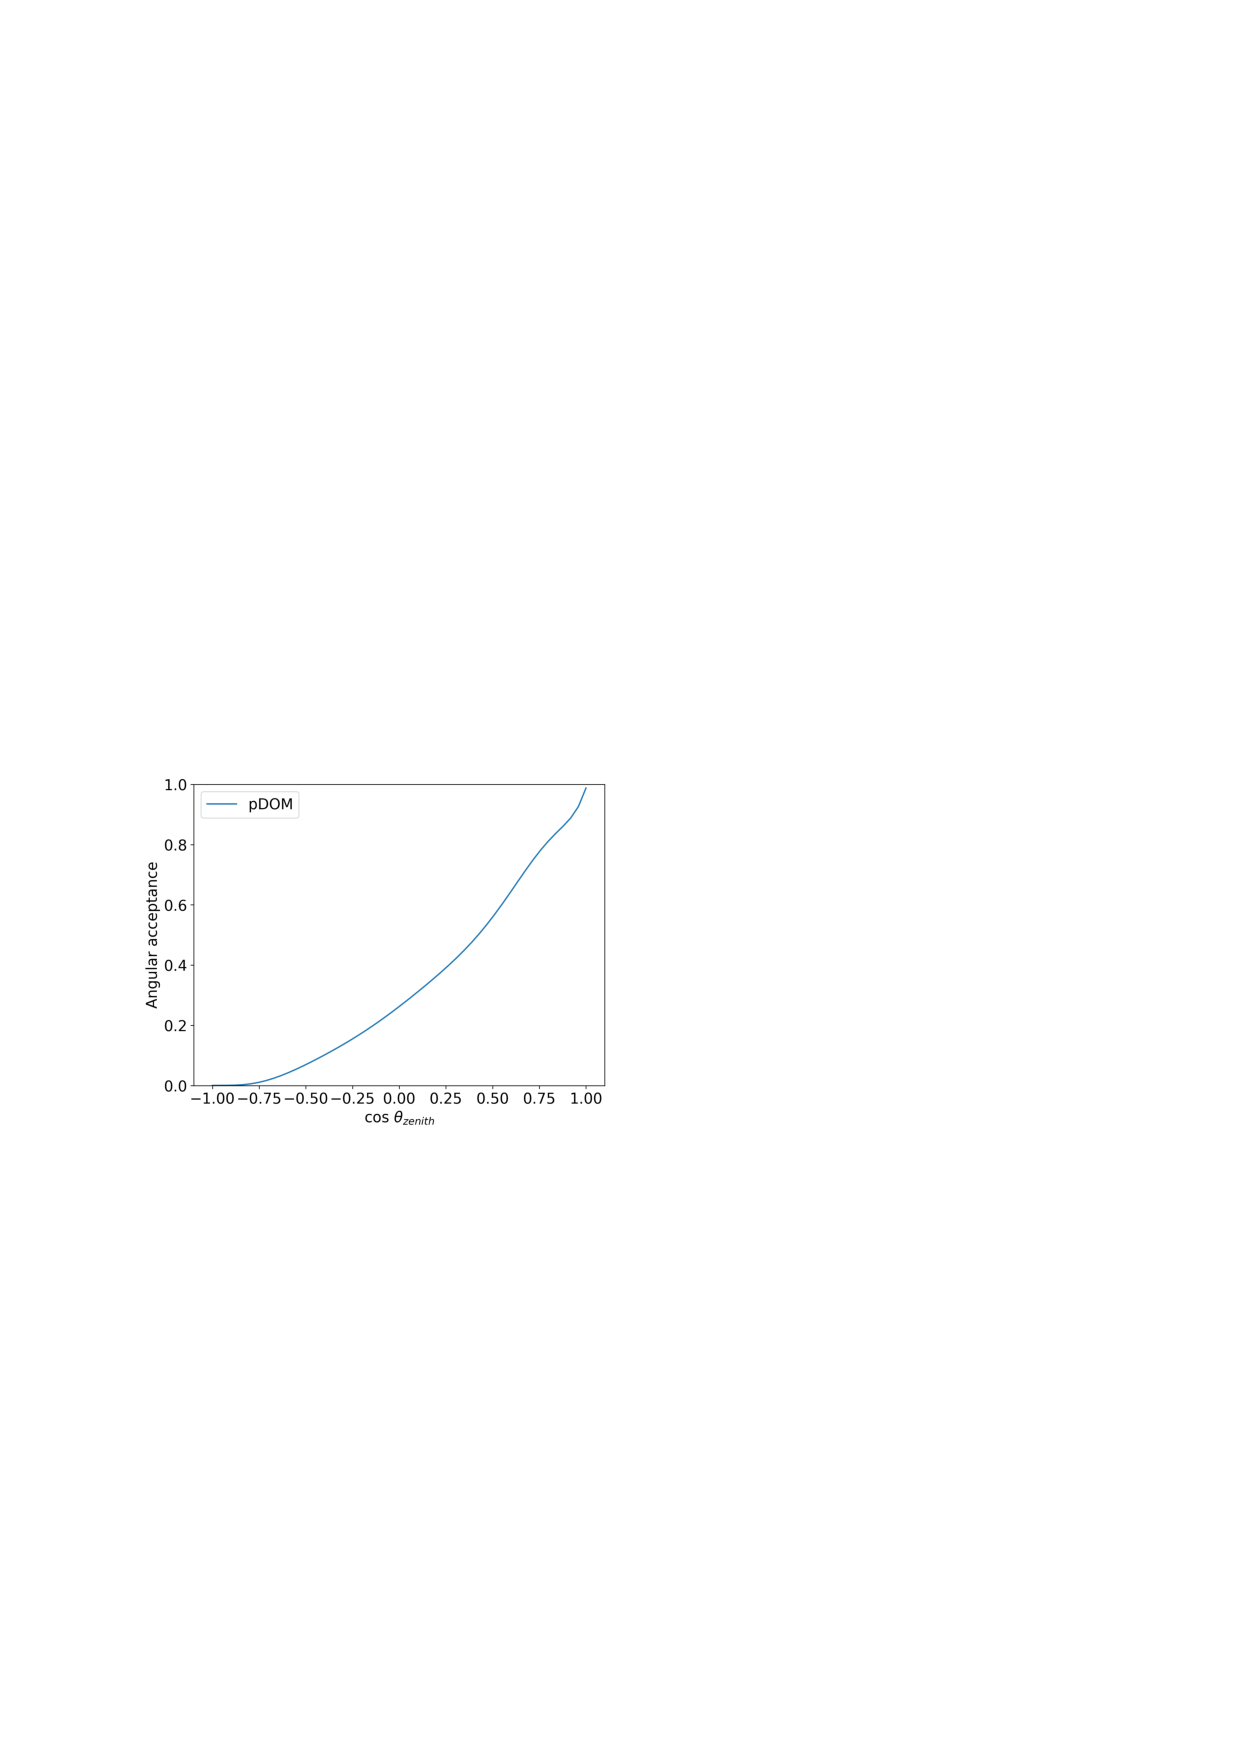
\includegraphics{./figures/gen2/ang_acceptance_curve.pdf}
%     \caption{Conceptual representation of Simulated sensor with isotropic angular acceptance (iso-pDOM) (reproduced from \cite{Anastasiia})}
%     \labfig{pdom_curve}
% \end{marginfigure}

% \begin{marginfigure}
%     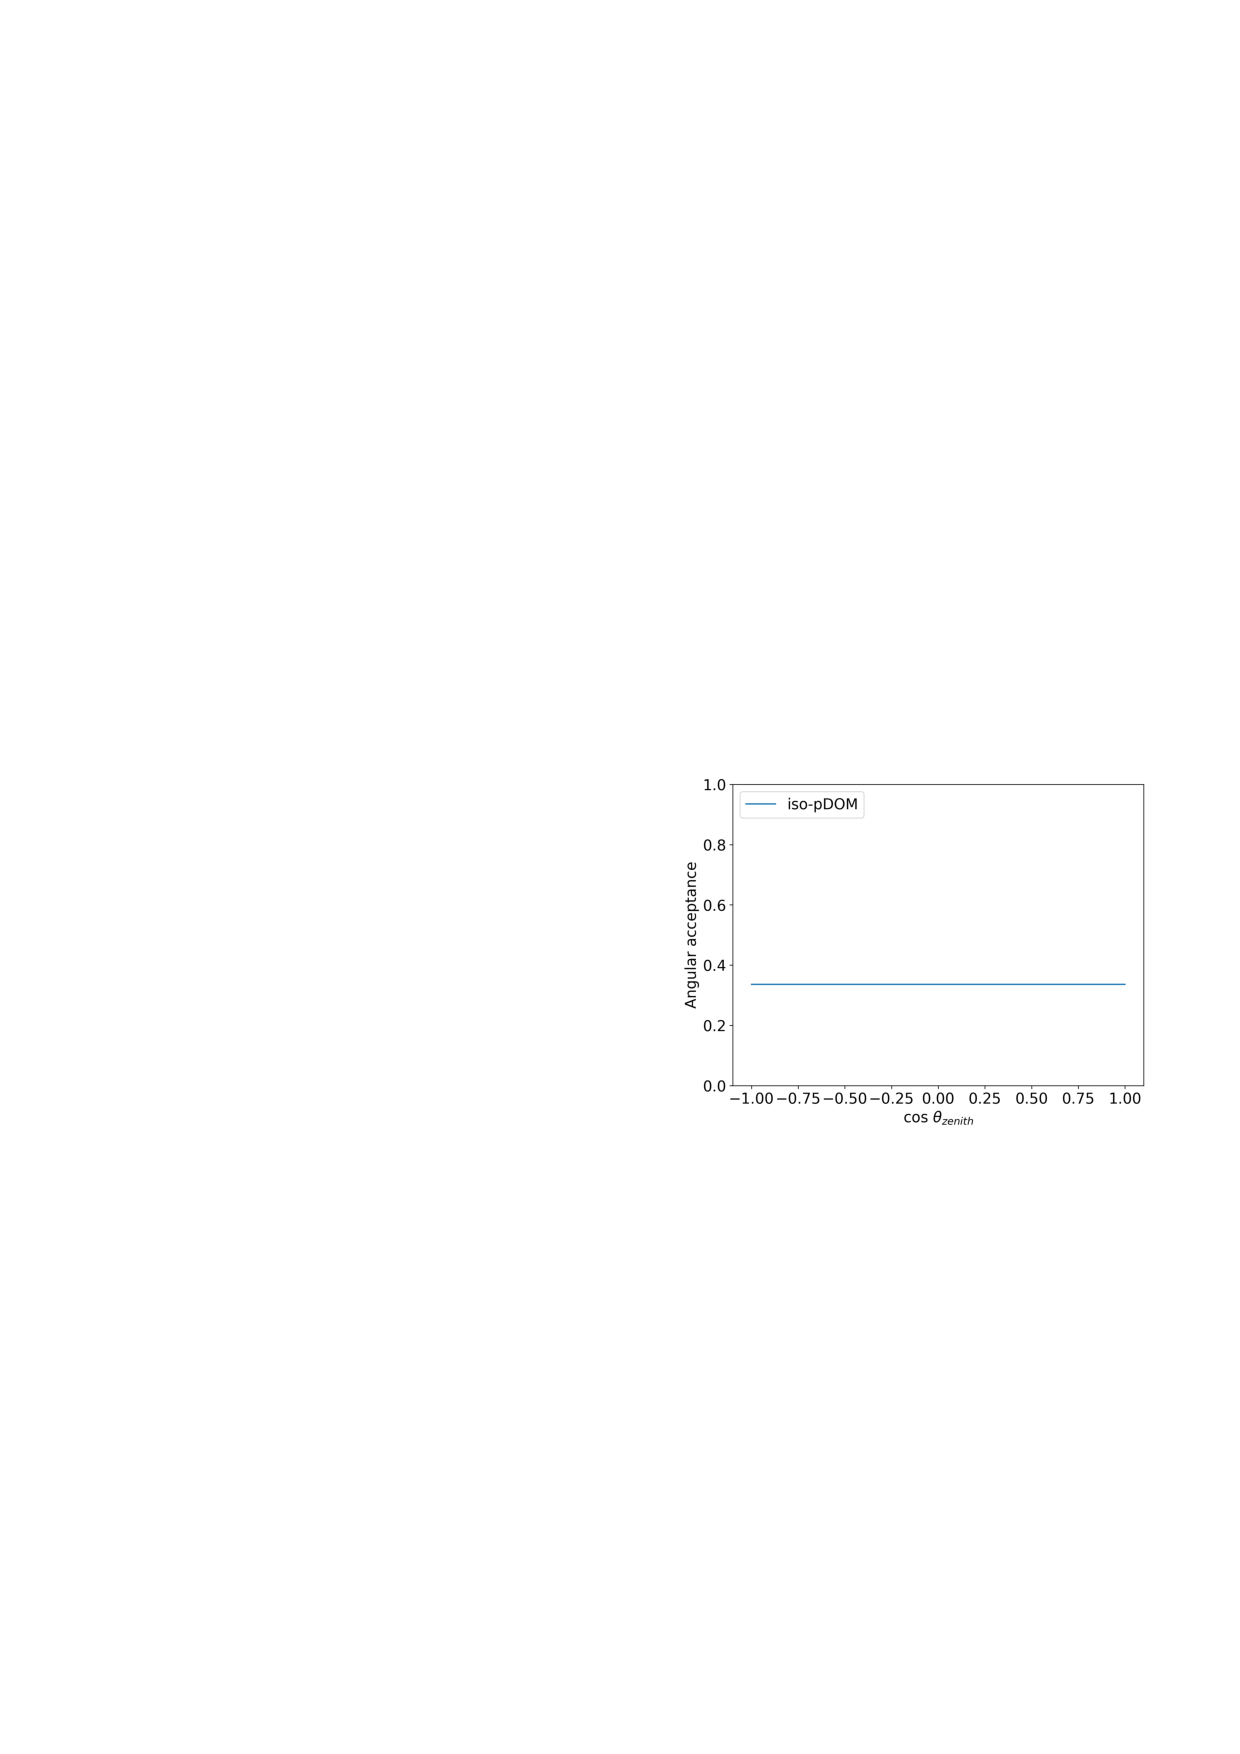
\includegraphics{./figures/gen2/ang_acceptance_isopdom.pdf}
%     \caption{Conceptual representation of Simulated sensor with isotropic angular acceptance (iso-pDOM) (reproduced from \cite{Anastasiia})} 
%     \labfig{isopdom_curve}
% \end{marginfigure}

However, all the existing sophisticated methods do not yet provide a full-scale simulated multi-PMT modules. Hence, a simulated sensor called \emph{isoPDOM} (isotropic-PDOM) is used. This sensor can be visualized as (see \reffig{isoPDOM_schematic}) a 'spherical PMT' housed in a glass vessel similar to an IceCube DOM but with 2.2 times higher quantum efficiency (or pDOM). 
% It is done by changing angular acceptance curve of regular pDOM, where acceptance is highest in the Since area under the both integrals remains the same, all  the other physics parameters remains the same, the resultant sensor hence \emph{mimics} the so called mDOM. 



\subsection{Event Selection}
\label{sec:gen2_eventsample}
Monte Carlo events were produced using the so-called isoPDOM for all three flavors of primary neutrinos with energies ranging from 100 TeV to 50 PeV. The simulation chain is identical to that described in \ref{nu_samples}. It is important to note that since the IceCube in-ice array is inherently part of the proposed Gen2 detector, all simulated events still include 'hits' from the IC86 configuration. Additionally, during the DetectorSim stage of the simulation chain, where PMT responses, noise, etc., are added, responses are incorporated separately for IceCube DOMs and isoPDOMs. If an event passes all the basic triggers, two separate triggers are stored depending on the event location: IC86 and ICGen2. By default, ICGen2 has a combined response of both detector configurations, while IC86 only contains current IceCube volume events. This feature is crucial as it facilitates direct comparison of events produced with IceCube simulations for IceCube-only analyses.


\section{Analysis Concept and tools}
\label{sec:gen2-software}




\section{Result of Flavour Sensitivity Measurements}
\label{sec:gen2-results}